\documentclass[11pt]{article}
\usepackage[brazilian]{babel}
\usepackage[utf8]{inputenc} %acentuação da língua portuguesa
\usepackage[T1]{fontenc} 
\usepackage{wrapfig} %figura ao lado do texto
\usepackage{graphicx} %pacote de figuras

\usepackage{amsfonts} %pacote com \mathbb{}

\usepackage[pdftex]{hyperref} %links da internet

\usepackage{fancyhdr} 

\usepackage{hyphenat} %retirar hefenação

\tolerance=1 %retirar hefenação

\emergencystretch=\maxdimen %retirar hefenação

\hyphenpenalty=10000 %retirar hefenação

\hbadness=10000 %retirar hefenação

\hyphenchar\font=-1 %retirar hefenação

\sloppy %retirar hefenação

\usepackage{textcomp}

\usepackage[a4paper,left=2cm,right=2cm,top=2.5cm,bottom=2cm]{geometry}

\setlength{\parindent}{0pt} %Parágrafo sem identação]

\begin{document}
	
\pagestyle{fancy}
\renewcommand{\headrulewidth}{0pt}
\renewcommand{\footrulewidth}{2.1pt}
\fancyfoot[L]{\small Diego Silveira Costa Nascimento}
\fancyfoot[R]{\small diego.nascimento@ifrn.edu.br}
	
\begin{minipage}[c][1.5cm][c]{3cm}
	\begin{flushleft}
		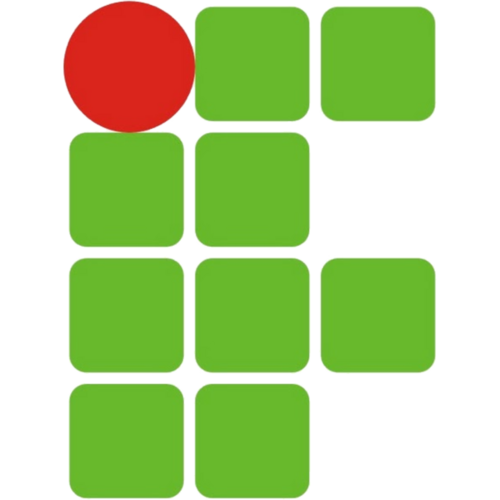
\includegraphics[scale=0.25]{IFRN}
	\end{flushleft}
\end{minipage}		
\begin{minipage}[c][1.5cm][c]{10.8cm}
	\begin{center}
		\resizebox{!}{0.3cm}{\textbf{Estrutura de Dados}}\par
		\resizebox{!}{0.2cm}{\textbf{Instituto Federal do Rio Grande do Norte}}\par
		\resizebox{!}{0.2cm}{\today}
	\end{center}
\end{minipage}

\section{Ordenação}

\begin{enumerate}

\item Implementar um programa que faça a ordenação de um vetor de 100 elementos gerados aleatoriamente via método Insert Sort.

\item Implementar um programa que calcule o tempo de ordenação de um vetor de 1000 elementos gerados aleatoriamente via método Insert Sort.

\item Implementar um programa que faça a ordenação de um vetor de 100 elementos gerados aleatoriamente via método Select Sort.

\item Implementar um programa que calcule o tempo de ordenação de um vetor de 1000 elementos gerados aleatoriamente via método Select Sort.

\item Implementar um programa que faça a ordenação de um vetor de 100 elementos gerados aleatoriamente via método Bubble Sort.

\item Implementar um programa que calcule o tempo de ordenação de um vetor de 1000 elementos gerados aleatoriamente via método Bubble Sort.

\item Implementar um programa que faça a ordenação de um vetor de 100 elementos gerados aleatoriamente via método Merge Sort.

\item Implementar um programa que calcule o tempo de ordenação de um vetor de 1000 elementos gerados aleatoriamente via método Merge Sort.

\item Implementar um programa que faça a ordenação de um vetor de 100 elementos gerados aleatoriamente via método Quick Sort.

\item Implementar um programa que calcule o tempo de ordenação de um vetor de 1000 elementos gerados aleatoriamente via método Quick Sort.

\item Implementar um programa que calcule o tempo de ordenação de um vetor de 2000 elementos gerados aleatoriamente via métodos Insert Sort, Select Sort, Bubble Sort, Merge Sort, Quick Sort, e exiba na tela o ranking dos tempo de cada método.

\end{enumerate}

\newpage
\section{Lista}

\begin{enumerate}
	
	\item Usando listas ligadas, implementar uma agenda telefônica contendo nome e telefone, que permita as operações:
	
	\begin{enumerate}
		
		\item Cadastro ilimitado de contatos
		
		\item Exclusão de contato a partir do nome
		
		\item Exclusão de um contato a partir de uma posição específica da lista;
		
		\item Recuperar o total de elemento da lista
		
		\item Listar todos os elementos da lista
		
		\item Procurar por um determinado contato na lista
		
	\end{enumerate}
	
	\item Implementar uma lista duplamente ligada.
	
	\item Implementar uma lista circular.
\end{enumerate}

\newpage
\section{Pilha}

\begin{enumerate}
	
	\item Implementar uma pilha que possua os métodos de empilhar e desempilhar.
	
	\item Escreva um programa para ler uma frase digitada via teclado, armazene cada letra em uma pilha, e como saída, exiba na tela a frase invertida.
	
	\item Escreva um programa que use pilha para verificar se uma data cadeia de caracteres é ou não palíndroma. Por exemplo: ``subi no onibus'' ou ``amor a roma'' é palíndroma.
	
\end{enumerate}

\newpage
\section{Fila}

\begin{enumerate}
	
	\item Implementar uma fila que possua os métodos de enfileira e desenfileirar.
	
	\item Implementar um programa que  simule uma fila de espera de uma clínica médica para os pacientes serem atendidos em ordem de chegada.
	
	\item Melhorar o programa da questão 2 para que a fila leve em consideração prioridade para os pacientes com mais de 65 anos de idade.
\end{enumerate}

\newpage
\section{Árvore}

\begin{enumerate}
	
	\item Implementar um programa que monte uma árvore binária numérica.
	
	\item Implementar um método de busca em profundidade dos elementos da árvore.
	
	\item Implementar um método de busca em largura dos elementos da árvores.
	
	\item Implementar um método para exclusão de elementos em uma árvore. 
	
	\item Implementar um método para fazer o balanceamento da árvore.
	
	\item Implementar um programa que monte uma árvore de taxinomia de animais.
	
	\item Implementar um programa que monte um árvore genealógica de uma família.
	
\end{enumerate}

\end{document}